%==================================================================%
% Author : Pando Muñoz, Manuel                                     %
%          Sánchez Barreiro, Pablo                                 %
% Version: 1.0, 30/03/2011                                         %
%                                                                  %
% Memoria del Proyecto Fin de Carrera                              %
% Archivo raíz para el capítulo de la arquitectura del sistema     %
%==================================================================%


\chapterheader{Arquitectura y diseño}{Definición Arquitectónica y Diseño Software}
\label{chap:arquitectura}

El presente capítulo \todo{finalizar breve introducción}

\chaptertoc

\section{Arquitectura física del Sistema}
\label{sec:arquitectura:arqFisica}

En esta sección se describe la arquitectura física del sistema mediante un diagrama de despliegue.
\begin{figure}
    \centering
    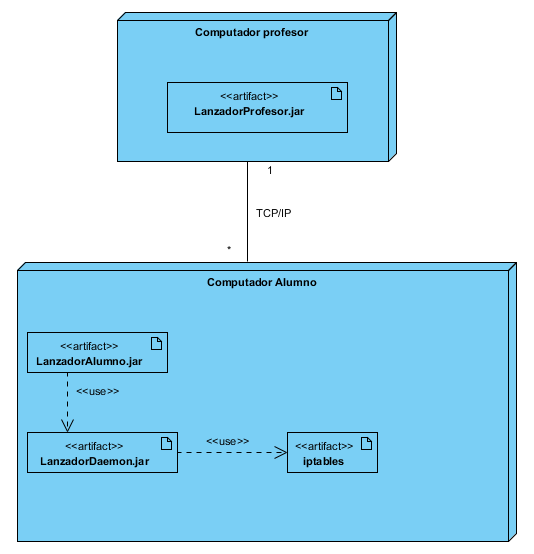
\includegraphics{arquitectura/despliegueSistema}
    \caption{Diagrama de despliegue del sistema}
    \label{fig:arquitectura:despliegueSistema}
\end{figure}
\newline

Cómo se puede puede observar, sólo se permite la existencia de una aplicación en el computador del profesor, a la que se conectan mediante TCP/IP un número indefinido de aplicaciones alumno, lógico, ya que en cada prueba suele haber varios los alumnos realizándola y uno el número de profesores.
\newline

Se ve también cómo la aplicación del alumno interactúa con un daemon del sistema que a su vez utiliza iptables para denegar o permitir el acceso a la red cuándo sea necesario.


\section{Diseño Software}
\label{sec:arquitectura:diseno}

En está sección se muestra un diagrama de actividad que resume las posibles interacciones que tanto el alumno como el profesor realizan con sus respectivas aplicaciones durante el trascurso normal de una prueba.
\newline

\begin{figure}
    \centering
    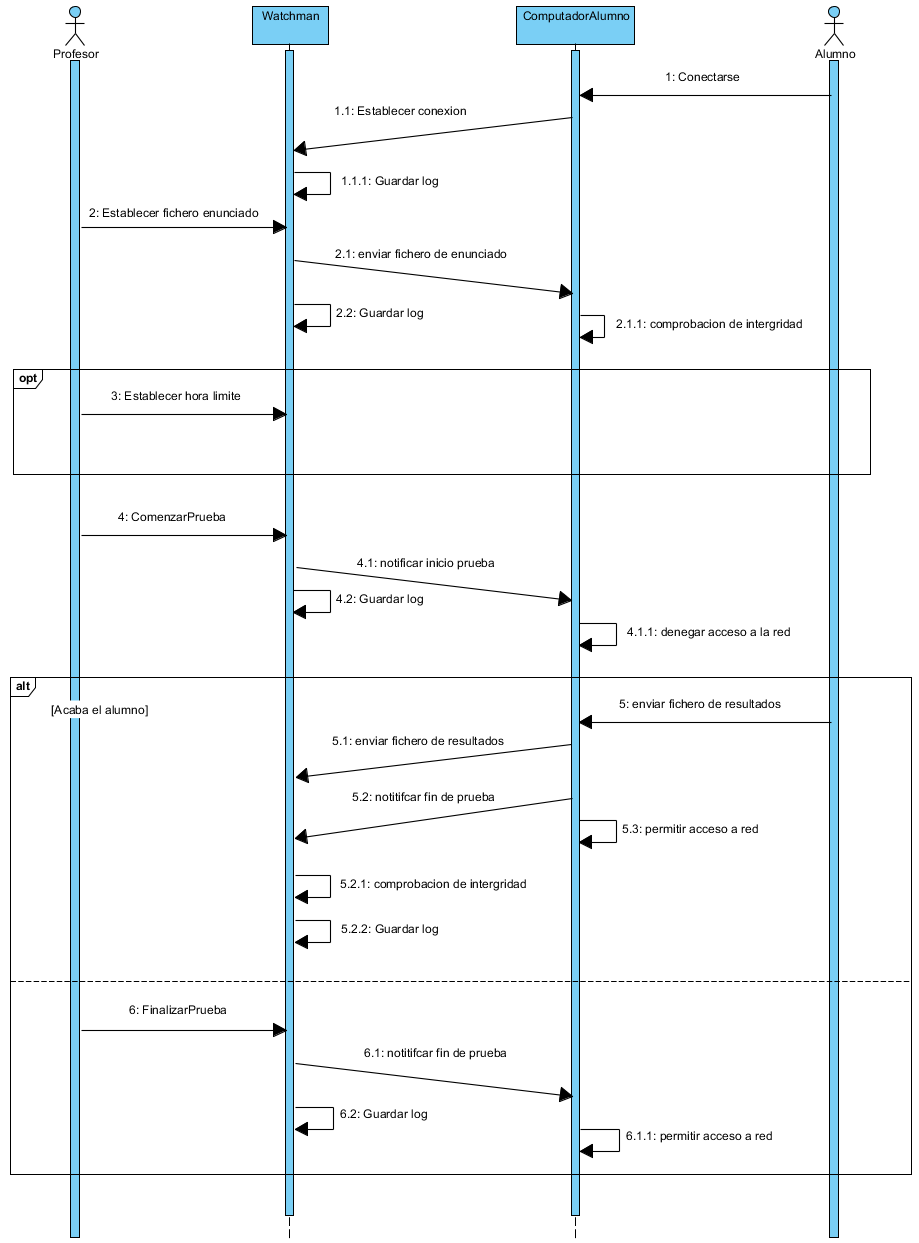
\includegraphics[width=12cm]{arquitectura/actividadSistema}
    \caption{Diagrama de actividad del sistema}
    \label{fig:arquitectura:actividadSistema}
\end{figure}


Vemos que se siguen los pasos descritos en la sección \ref{sec:planificacion:descFuncional}


\begin{figure}
    \centering
    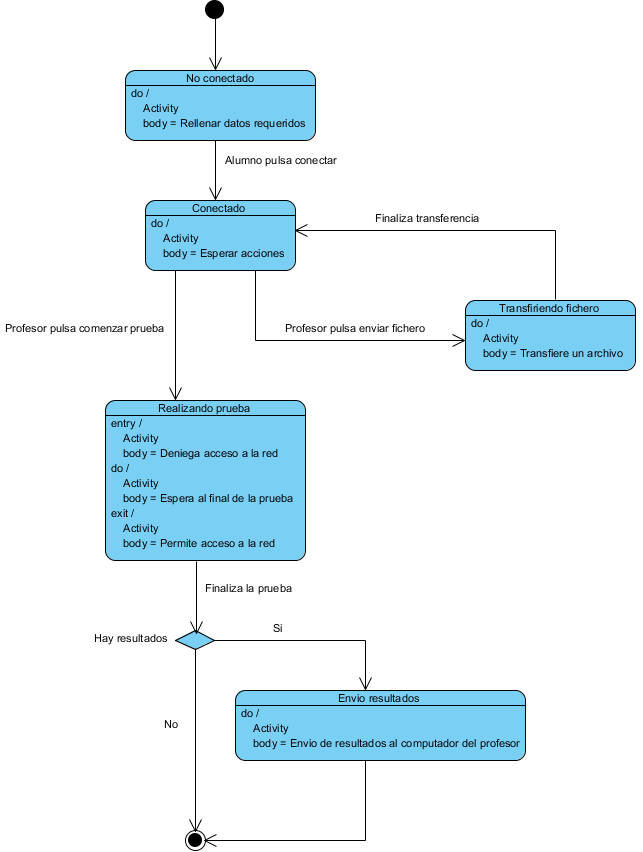
\includegraphics[width=12cm]{arquitectura/estadosAlumno}
    \caption{Diagrama de estados de la aplicación del alumno}
    \label{fig:arquitectura:estadosAlumno}
\end{figure}



%% Razonar porque el software es seguro
La principal funcionalidad de la aplicación es la de denegar el acceso a la red en los computadores de los alumnos que están realizando la prueba, mientras la prueba esté en marcha, sin necesidad de apagar el router o switch del laboratorio. Esto se consigue por medio de iptables, cambiando la política de los paquetes salientes una vez que empieza la prueba y hasta que acaba.
\newline

Por defecto iptables permite todo el tráfico que entre y salga del equipo, modificando las reglas para que deseche cualquier paquete destinado a cualquier equipo, conseguimos que no se pueda realizar ninguna petición a ningún nodo de la red, y, por tanto, tampoco recibiremos el contenido de la posible respuesta, el equipo del alumno queda aislado del resto.
\newline

A la hora de volver a permitir el acceso a la red, basta con modificar la política para el tratamiento de los paquetes salientes y restaurarla al estado anterior. Un alumno corriente no puede realizar esta operación ya que son necesarios privilegios de administrador para ello.
\newline

Otro punto importante es el de la recogida de resultados automática, se ha de garantizar que el archivo no se ha corrompido a lo largo de la transferencia, para ello se realizan, tanto en el equipo que envía el fichero como en el que lo recibe, firmas MD5 al mismo para comprobar que no ha habido errores en la transferencia.
